% https://www.overleaf.com/6622695572gyrgqvhzstkh

\documentclass{article}

%\documentclass[conference]{IEEEtran}
%\def\BibTeX{{\rm B\kern-.05em{\sc i\kern-.025em b}\kern-.08em
%    T\kern-.1667em\lower.7ex\hbox{E}\kern-.125emX}}
\usepackage{xcolor}    
\usepackage{graphicx} % Allows including images
\usepackage[backend=bibtex,style=verbose-trad2]{biblatex}
\bibliography{bibfile} 


\begin{document}

%%%%%%%%%%%%%%%%%%%%%%%%%%%%%%%%%%%%%%% TITLE %%%%%%%%%%%%%%%%%%%%%%%%%%%%%%%%%%%%%%%%%%%%%%%%%%%
%%\color{blue}

\title{caDDS: Community Assisted Distributed Database for Sequences}

\author{\IEEEauthorblockN{1\textsuperscript{st} Carl Araya}
\IEEEauthorblockA{\textit{Algorithms and Complexity Laboratory } \\
\textit{Philippine Genome Center}\\
\textit{University of the Philippines - Diliman}\\
Quezon City, Philippines \\
jjazcarraga@up.edu.ph}
\and
\IEEEauthorblockN{2\textsuperscript{nd} Cid Azcarraga}
\IEEEauthorblockA{\textit{Algorithms and Complexity Laboratory } \\
\textit{Philippine Genome Center}\\
\textit{University of the Philippines - Diliman}\\
Quezon City, Philippines \\
jjazcarraga@up.edu.ph}
}

\maketitle

%%%%%%%%%%%%%%%%%%%%%%%%%%%%%%%%%%%%%%% INTRODUCTION %%%%%%%%%%%%%%%%%%%%%%%%%%%%%%%%%%%%%%%%%%%%%%%%%%%

\section{Introduction}
%(done)CID: Start the idea that inside each body is the following:
Inside every human body are the instructions to create and maintain it. These instructions are found inside the genome. The entire human genome, when laid out is around 2 meters in length. \autocite{ency_sci_tech}
%(done) KING: cite this
But once all of the DNA of all the cells in the human body are combined. The length can span the earth to moon 6000 times. This shows the length and amount of DNA inside the human body. This describes as well the vast amounts of information in the body. 

%CID: Add a paragraph elaborating further on the amount of information here.

%(partial done) CID: This intro lacks references and needs better visual description

The word \textit{genome} was used briefly. But first, what does genomes or genomics actually mean?

\subsection{Definition}
National Institute of Health \autocite{genomics-definition} defines genomics as \\ \\
\textit{Genomics is the study of all of a person's genes (the genome), including interactions of those genes with each other and with the person's environment.} \\ \\

%(partially done) CID: Mej abrupt pagpasok kaagad sa genomics na definition. Walang clean transition

In the definition, there was also a word called genes. But what are genes? Genes comprises of DNA. DNA is an acronym that stands for deoxyribonucleic acid. DNA is usually characterized by the letters A,T,G,C. Where A is for Adenine, T is for Thymine, G is for Guanine, C is for Cytosine. These are the instructions passed on from one generation to another, this is also what is used to form the organism. \autocite[p.~2]{hartl2018}

%CID: Explain what the acronym DNA means. Then describe why that acronym becomes ATGC

These nucleotides
%(done)KING: Bases are the nucleotide
%CID: Explain this part more, it doesnt really explain the importance
form the base pairs (or \textit{bases}). These bases act as a blueprint to describe and instruct the body on how to build it and function.\autocite{alberts_mole}
%CID: Expound this sentence more, perhaps explain the build and functioning process

There are these components, and these describe complex organisms. Which means there is a long set of instructions to detail these complex organisms. For humans, the full human genome contain around $3.2x10^9$ base pairs \autocite{introgenomics}. This is a lot of information inside the human organism. But before analyzing that information, these have to be taken from the cells and read.

%CID: Separate the paragraphs to explain what genes are, to the paragraph explaining the complexity of the human genome (also elaborate on this)



\subsection{Sequencing}

%(partially done) CID: Have a clear transition to sequencing, you ended at complexity.
To see the information of the DNA of a cell. There are machines called \textbf{Sequencers} that look (or more appropriately, \textit{read}) the DNA of a specimen and outputs A,G,C,T. Sequencers look at the exact order of a single strand of DNA. The process of sequencing DNA isn't a simple process of a machine reading one strand of DNA. In most cases, one strand is too little for one machine to read. So before reading, the DNA is replicated multiple times in the laboratory. DNA is also fragmented before processing. Fragmented meaning it will be cut up into pieces.

%CID: Describe what fragmented means

These are fragmented since the machine cannot handle reading the entire length of the DNA, it has to read it in parts. Sequencers then reads (or sequences) them.  These reads of fragments from the replicated DNA will then be put back together computationally to form the \textit{correct or reference} DNA.

%CID: The paragraph on sequencing is good. Maybe cite more.


Back in 2003 The first human genome \autocite{introgenomics} had been first completely read. It took the project ten years of work, a dozen institutions, and 3,000,000,000 dollars to finish. Currently, in 2019, the technology today in Japan is much faster than the technology back in 2003. The technology in Japan can read 10,000 human genomes per day. \autocite[p.~19]{introgenomics} 
%(done) KING: Cite


% (partially done) CID: Get the transition of the NGS data graph from the slides

\begin{figure}[h]
\caption{Cost per Genome Data Over Time}
\centering
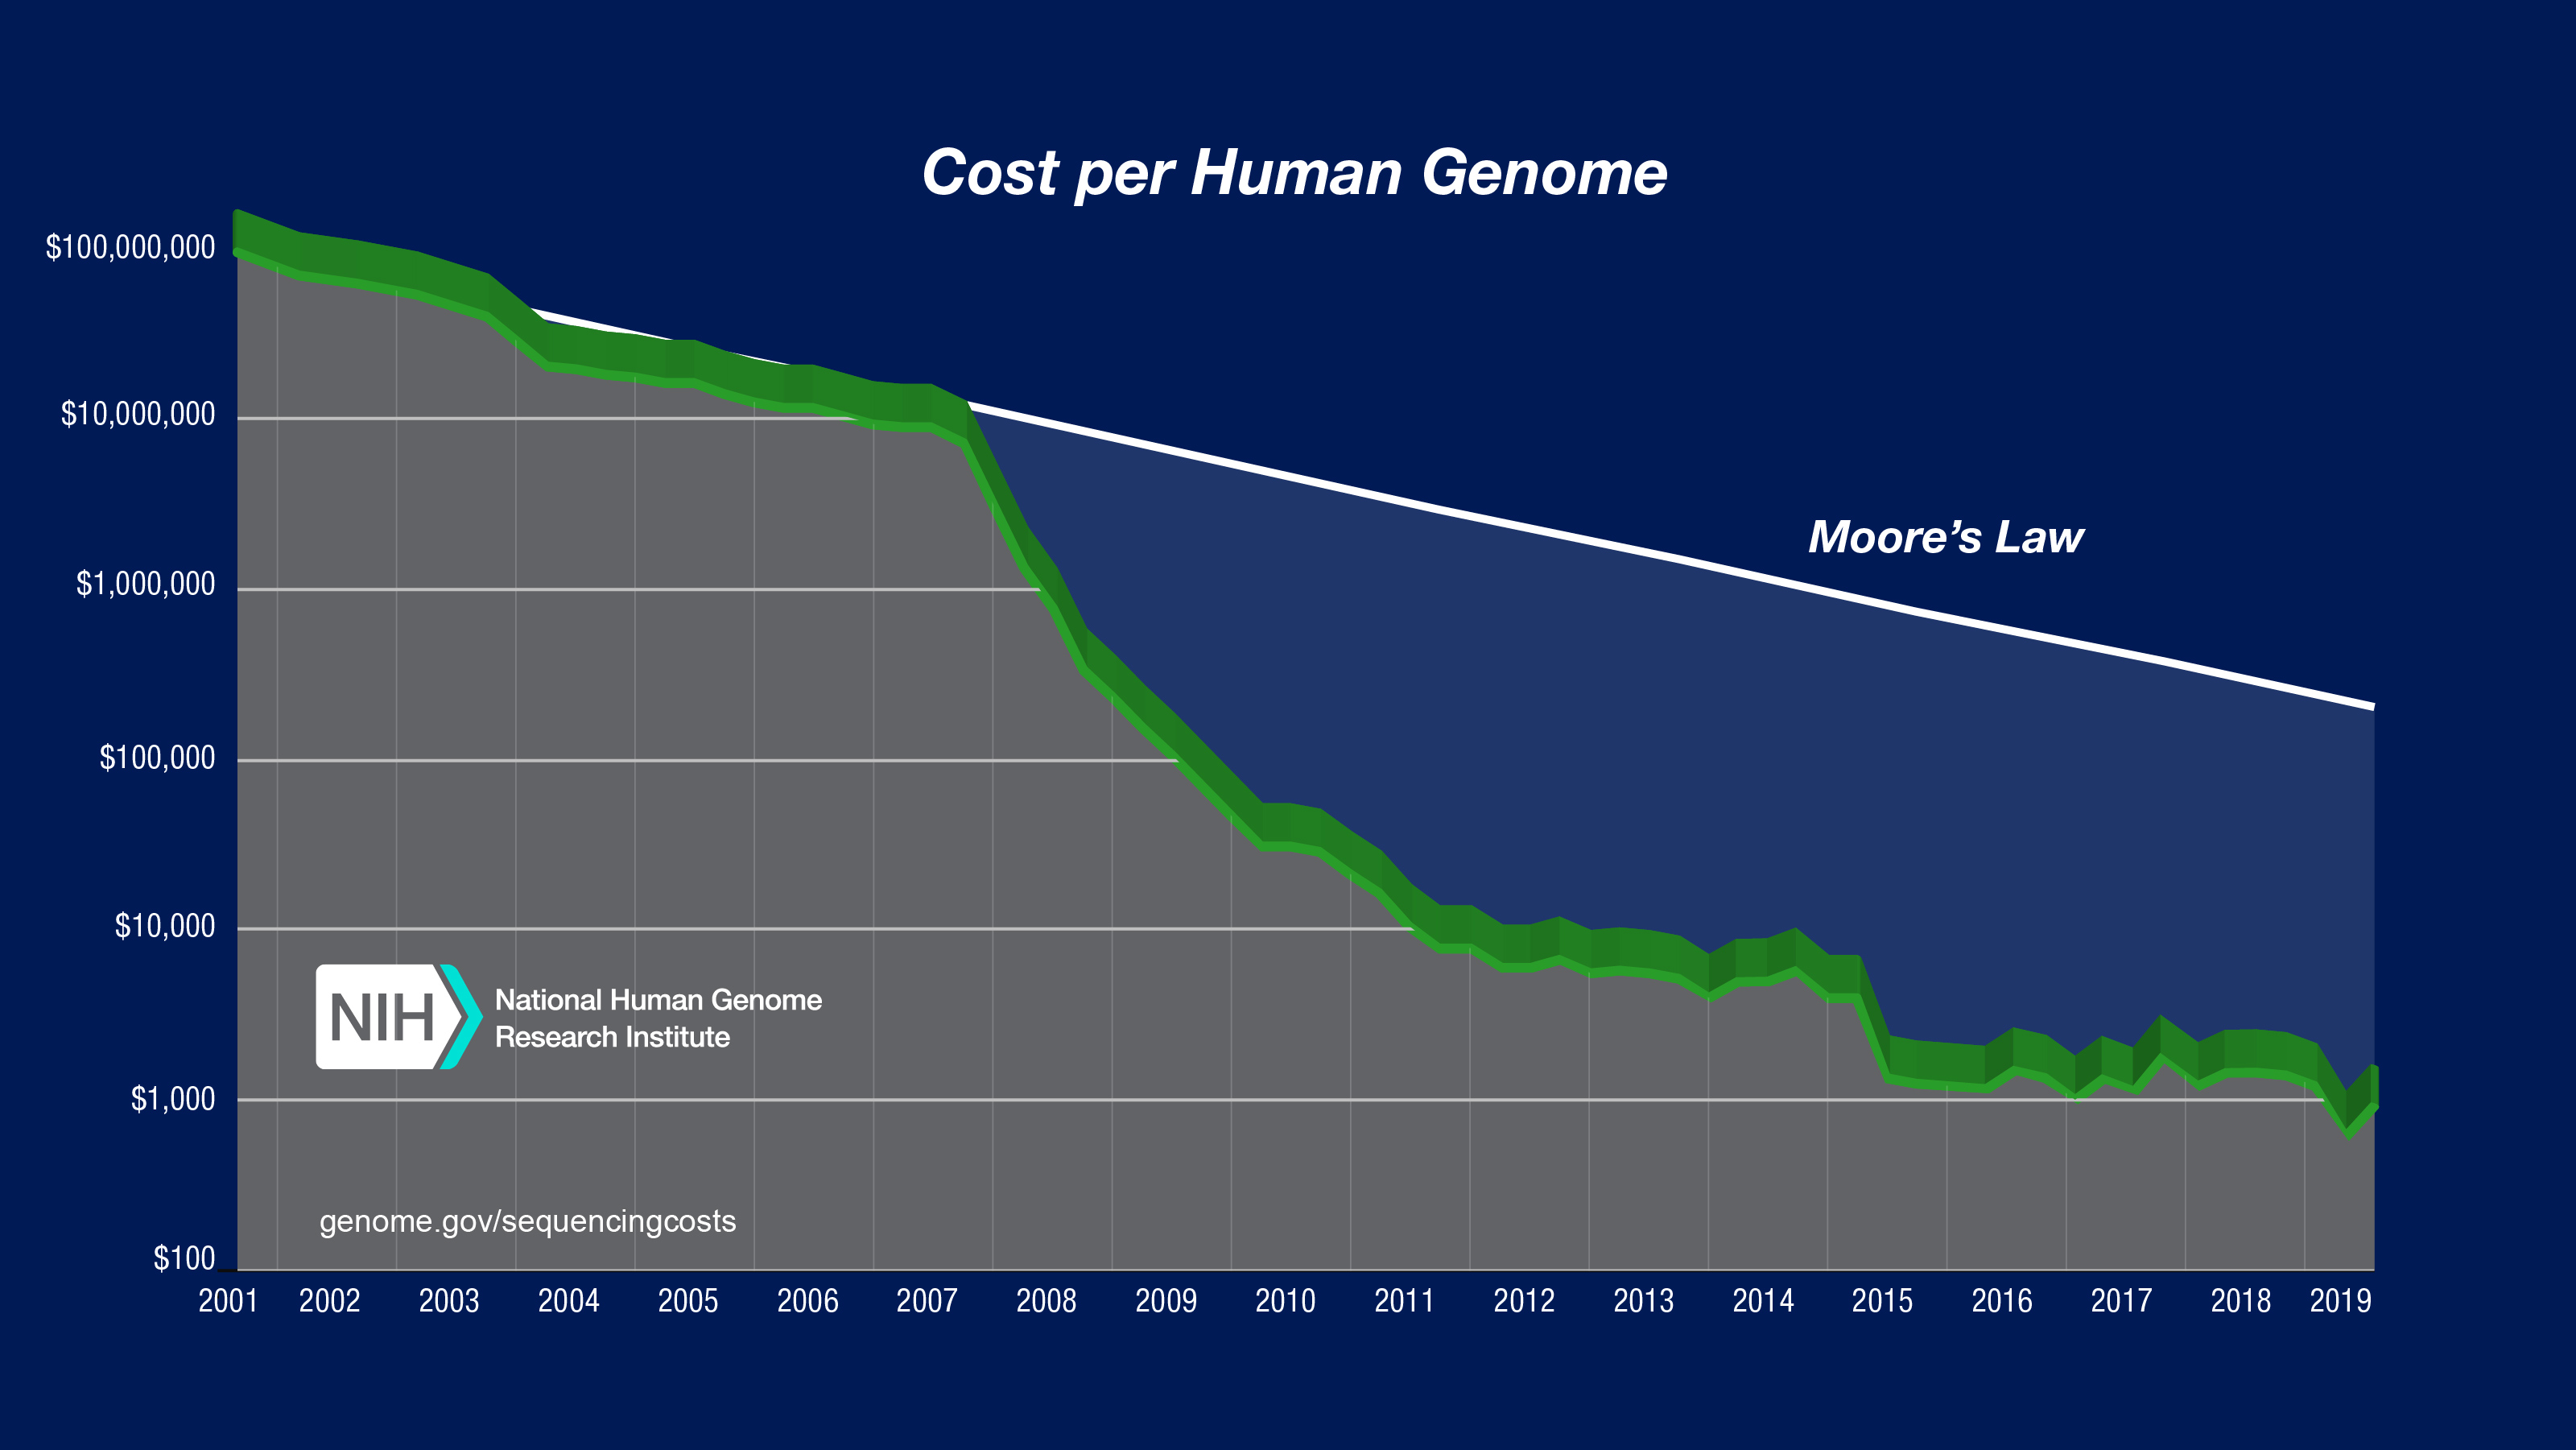
\includegraphics[width=0.65\textwidth]{images/human-gen-cost.jpg} 
\label{fig:human_gen_cost_fig}
\end{figure}

Looking at the Figure~\ref{fig:human_gen_cost_fig} on Page~\pageref{fig:human_gen_cost_fig} \autocite{genomics-cost}, we note the expensive cost at the initial stages of sequencing the human genome. But as time progresses, the cost substantially went down to what it is now. The big fall of the prices around 2004 - 2005 corresponds to the introduction of the Next Generation Sequencers.


\subsubsection{Next Generation Sequencing}

%(done) CID: Describe the speedup in terms of what and how the speedup was computed

The introduction of Next Generation Sequencers can be seen as a significant event in the history of genomics. This is a new technology which has allowed the machines to read faster and cheaper. These utilize a variety of technologies, some make use of light, some use ion semiconductors, others use a special DNA marker with a fluorescent probe \autocite[~p.67]{paulselzer2018}. This tech has increased the read speed and speed in which data is produced. But note as the data increases, storage demand therefore also increases. Since each read requires storage. This poses a problem to projects involving sequences, the data volumes is usually very large\autocite{bon_compression}. There exists a concept of \textit{coverage} as well. It means the number of reads it needs in order to produce a reference sequence (the correct, standard sequence). Meaning the sequence isn't read only once. This contributes to the large data size of sequences. Currently, for a coverage of around 60, the file size for a compressed human genome can easily reach 200 GB. And a project of 10-20 genomes would need approximately 4 TB of storage. Transferring these data across research groups would indeed be a challenge. \autocite[~p.68]{paulselzer2018}
%(done) KING: cite
% more space is used.

%(done) CID: Visually explain how more space is needed (cite numbers). May separate the sentences describing NGS and space utilization


\subsection{Database}

\begin{figure}[h]
\caption{Megabase Cost Over Time}
\centering
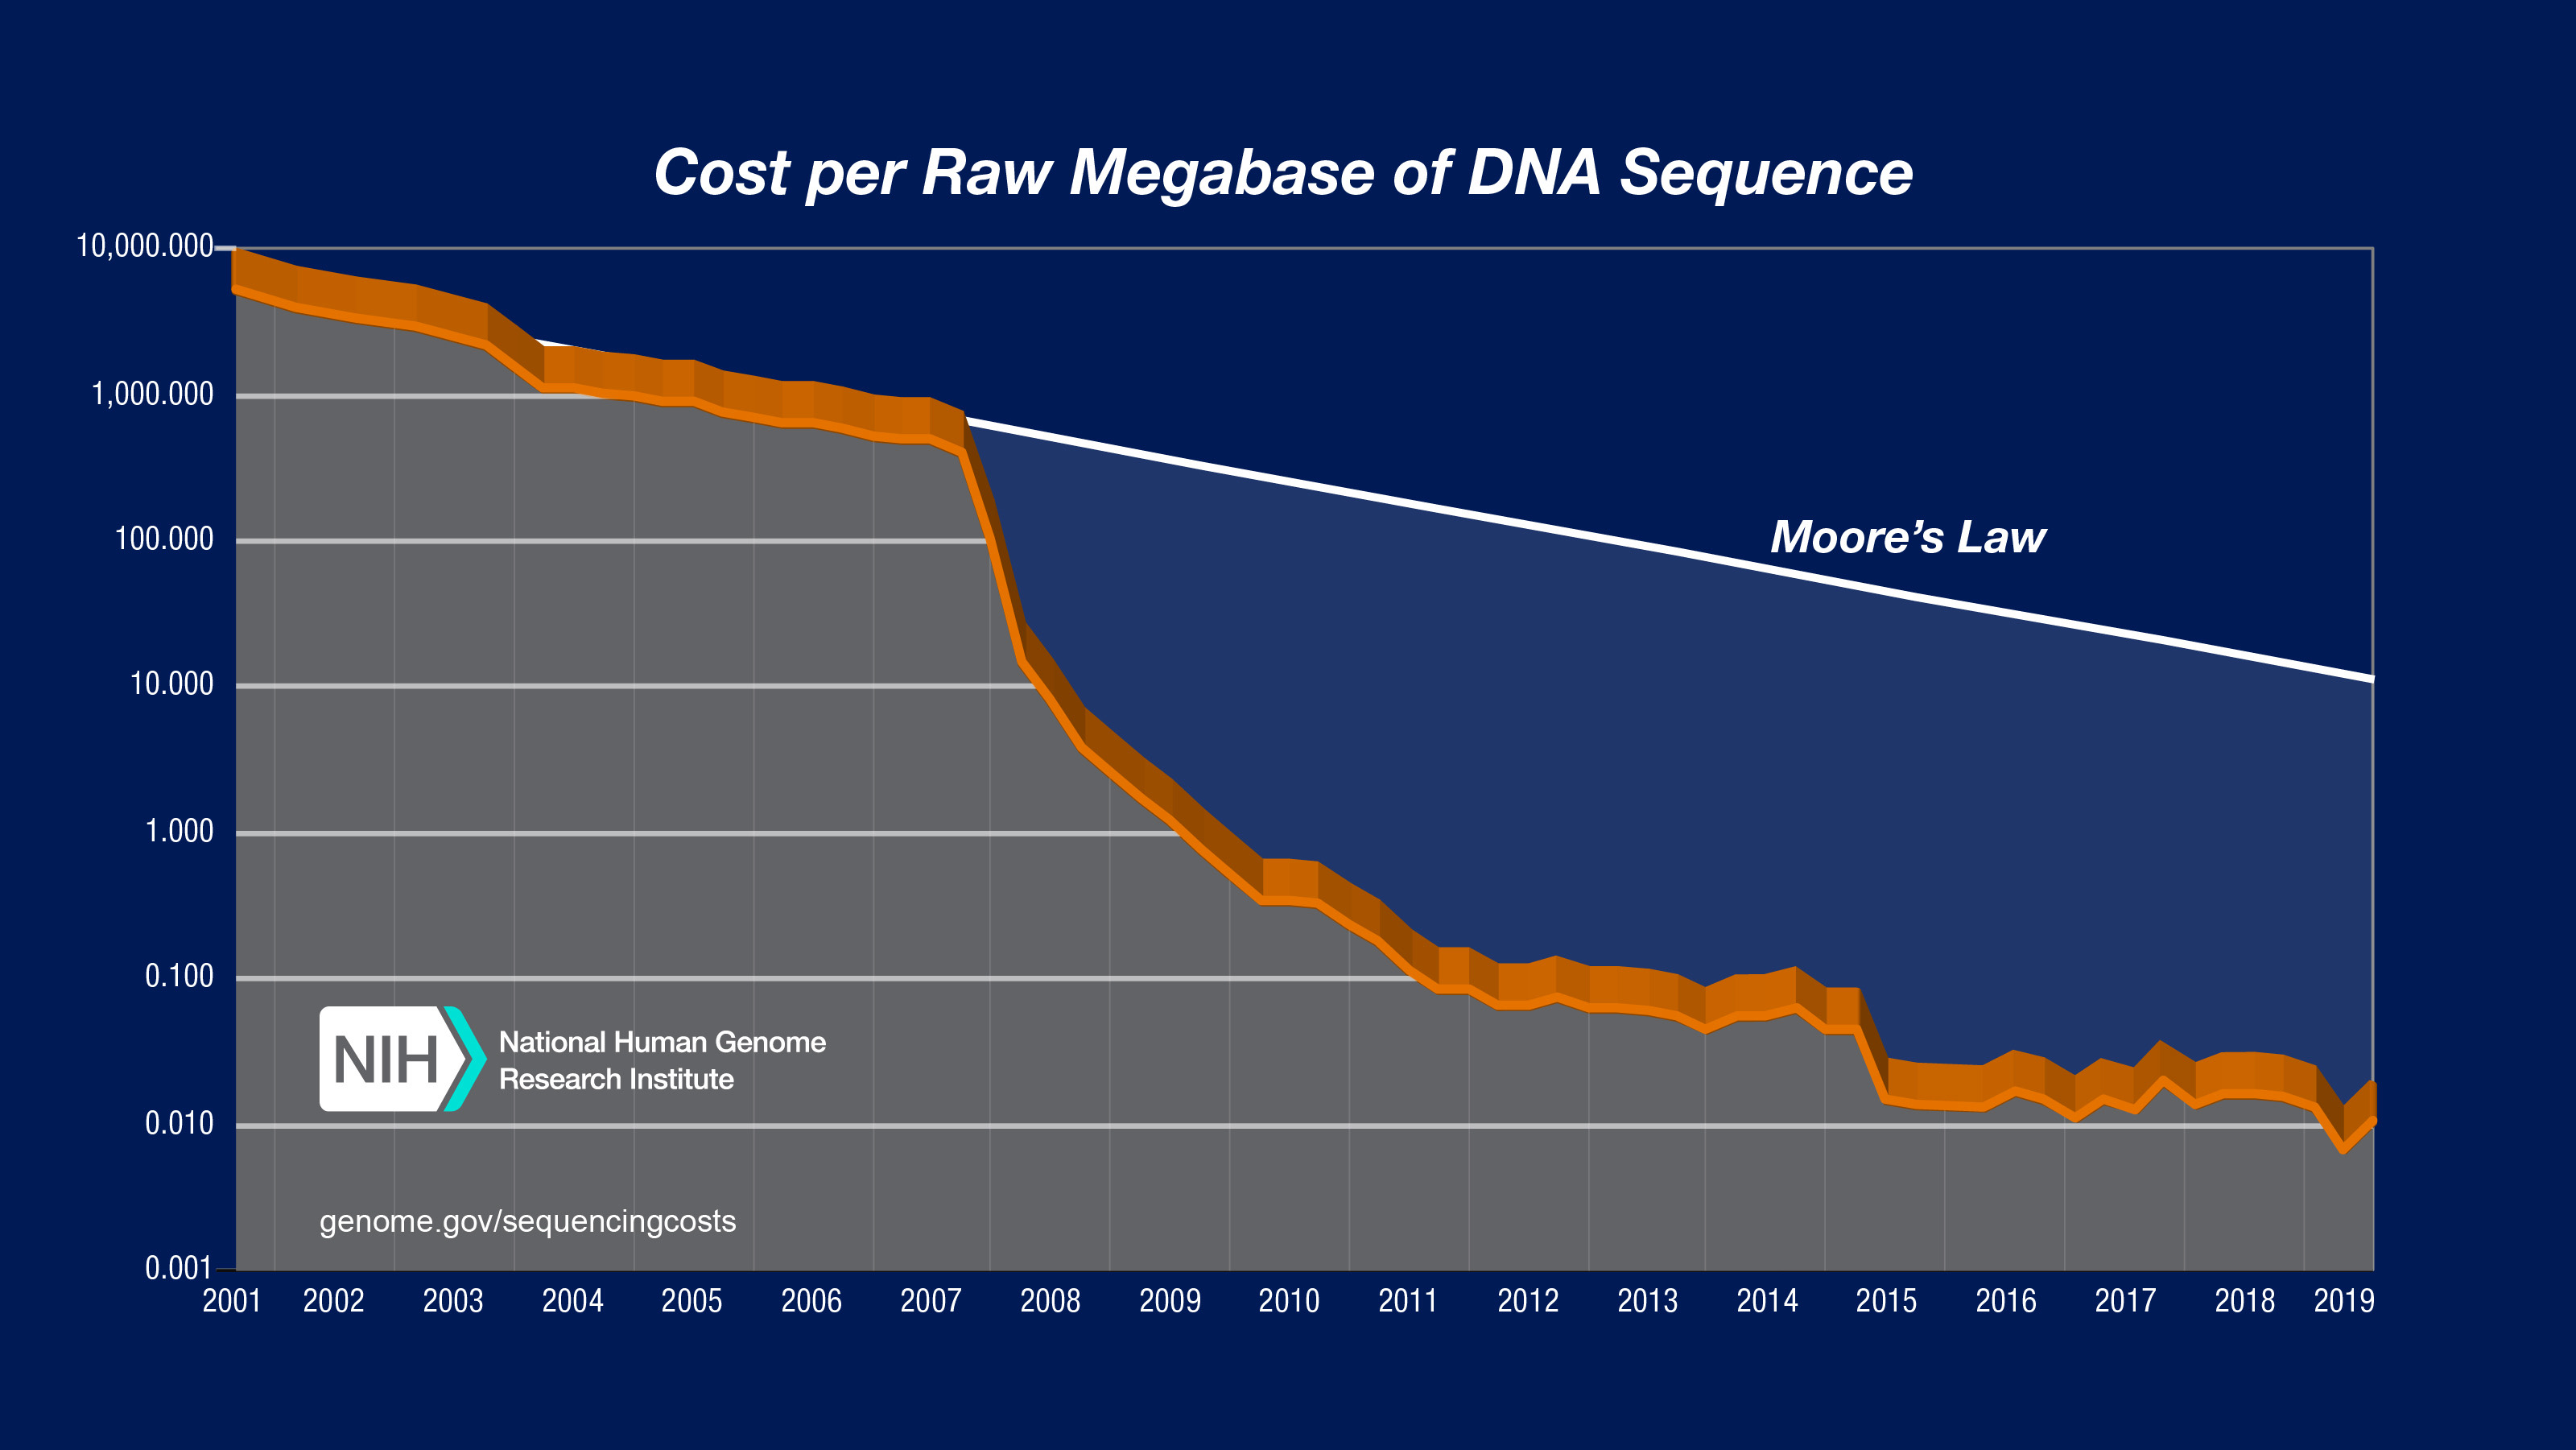
\includegraphics[width=0.65\textwidth]{images/seq-cost.jpeg} 
\label{fig:megabase_cost_fig}
\end{figure}

Similar to Figure~\ref{fig:human_gen_cost_fig} on Page~\pageref{fig:human_gen_cost_fig}, we also note the same pattern for the cost of sequencing (not just humans) in Figure~\ref{fig:megabase_cost_fig}\autocite{genomics-cost}. The cost of sequencing dropped 1000 fold from 2008 to 2012 alone \autocite{bon_compression}. This lowering of cost, makes the idea of sequencing more available. And thus produces a lot more data. But these terabytes of data need to be stored somewhere. 
 
\begin{center}
\textit{Moore's law states that the number of transistors on a chip doubles every two years.}
\end{center}

%CID: An idea: make a quote stating Moore's Law, cite, then explain how this relates to thesis
%KING: Cite and check if true

This means, that as time passes by, technology for processing and storage will improve. And the overall capacity for what technology can do will increase as well. But the speed in which the number of sequence data increases seems to exceed Moore's Law. And this will pose a problem since the technology doesn't seem to be catching up. The immediate problem is the storage of all the data being produced. A certain technology needs to be made for the purpose of holding this data. This technology is referred to as Databases. 

%CARL: change "flow" of ideas, maybe reorder/rewrite subsection names
% currently, the subsections are:
% - Database
%   - Principles
%   - Database Types
% - App Archi
%   - CS
%   - P2P
%   - Hybrid

\subsubsection{Definition}
A database (DBMS, Database Management System) is defined by containing information about a particular enterprise. Functionalities include: \autocite{Silberschatz2010}
\begin{itemize}
    \item Collection of interrelated data
    \item Set of programs to access the data
    \item An environment that is both convenient and efficient to use
\end{itemize}

These form a system that is made for accessing and updating data. 

%CID: Summarize a bit on why this was discussed and why this is needed in the thesis

\subsubsection{Principles} 
There are also 3 principles to remember when creating a database. The idea is that only 2 of the three can be focused on at any given time. And these need to be taken into consideration when designing the system. \autocite{Silberschatz2010}

\begin{itemize}
    \item Consistency - Update one part, will all other (replicated) parts be updated quickly as well; Data is accurate and copied faithfully. An example would be that genes for specimen A, when copied to another data node should contain the exact copy of the data, with no minor changes.
    \item Accessibility - How easy it is to access data, API protocols. An example would be the number of commands  a user needs to do to access every data.
    \item Partition Tolerance - If one portion breaks, the other portions are still usable. An example would be a power failure for one data node, how would this affect the other nodes?
\end{itemize}
%CID: Use explanations from the slides
%CID: Explain CRUD

\subsubsection{Database Types} 
Two types of databases will be discussed in this paper. Some of these databases will use technical terms, these terms will be discussed later in the Theoretical Framework. Namely: \autocite{centralizedvsdistributed}

\begin{itemize}
    \item Centralized - In a centralized database, all data are managed by a single DBMS in a single node to be distributed to users. As a result, transactions are easily manageable because everything can be processed in the single node, but the cost of communication is high and reliability is low, as an error in the database will mean disaster to the network as a whole.
    \item Distributed - In a distributed database, data are stored in multiple servers in different geographical locations. Each node may contain a part or the entirety of the data. The difficulty of managing transactions will go up, but the result is higher availability, faster response, and modular growth, among other advantages. 
\end{itemize}

%\begin{itemize}
%    \item Client-Server Database - Utilizes a client-server architecture. One server to sends and receives the data to all the clients. 
%    \item P2P Database - Utilizes a peer architecture. Each peer has the ability to send and receive the data to all the other peers. There is no hierarchy.
    
    %KING: One server that sends
    %KING: One server for sending
    %KING: One server sends
    %CID: Basically reexplain client and server architecture, wha does client mean, what does server mean
    
%    \item Hybrid (Or Distributed) Database - Utilizes master node and data node. Unlike the normal database, this maintains a different structure, where not only one server has all the data. And a concept of replication of data is happening.
%\end{itemize}

%CID: I dont see any problems here, perhaps cite nalang a bit more

%CID: Explain muna P2P CS H in intro.

\subsection{Application Architecture}
The application architecture is how a networked app is structured
across the various end systems (i.e. computers, servers, etc.) \autocite{kurose}
Falls into either client-server, peer-to-peer, or hybrid architecture
%CID: Explain a bit how application architecture affects the app? Like does this change the features or speed or traffic management?


\subsubsection{Client-Server}
A client-server architecture relies on a Web server that is always
available and has a fixed IP address. When a client sends a request for data, the server responds by sending the requested data. The client-server architecture may not be able to keep up with the increasing number of connections.

\subsubsection{P2P}
A peer-to-peer (P2P) architecture has minimal to no reliance on
always-on, dedicated servers. Peers are desktops/laptops that communicate to each other without passing through a dedicated server. These include internet telephony, BitTorrent, and some other file sharing protocols. An advantage of P2P networks is their scalability. Each user can benefit the whole network by sharing his/her own resources. However, P2P has its own problems, namely security and incentivizing users to share their resources.

\subsubsection{Hybrid}
A hybrid architecture combines elements of P2P and client-server architectures, attempting to utilize advantages of both.

%CID: Explain some problems din kaya?
%CARL: wala sa kurose eh what if gusto ko magdagdag ng sarili ko haha

%KING: Fix periods in a sentence

% this is only a particular implementation of hybrid kasi so cinomment out ko
 %A master node stores metadata of all sequences, may or may not contain sequence files. Data nodes stores sequence files and metadata of all sequence files in its filesystem. Both master node & data nodes have user interface that allow users to upload, search, and download sequence files.


%%%%%%%%%%%%%%%%%%%%%%%%%%%%%%%%%%%%%%% RRL %%%%%%%%%%%%%%%%%%%%%%%%%%%%%%%%%%%%%%%%%%%%%%%%%%%

\section{Review of Related Literature}

We review the technologies on data storage done before. 
%CID: Make a transition to go from the diff database types to the explanation of the diff databases

\subsection{SeqTorr: A distributed scalable database for genomic information}
The standard genomics workflow consists of uploading and downloading data on an international database like NCBI. Having a distributed scalable local infrastructure to store genomic data instead of relying on NCBI would be beneficial since: only certain sequences in NCBI are relevant to the institutions (e.g. Asian sequences are needed more than Caucasian ones), researchers within the country can share data with fast speeds, and  institutions can share in the hosting of data.

SeqTorr consists of a master node and multiple data nodes. The master node contains metadata of all the sequences and is where the user authentication is handled, while the data node is where the actual sequences are stored. All user uploads happen in the master node. When the master node receives a sequence from a user, it distributes the sequence to any available data nodes. 
\autocite{seqtorr}

Currently, SeqTorr is not available, and the code base does not have any documentation which makes future work difficult.



\subsection{BioTorrents}
Scientific data continues to grow, and so does the demand for easier accessibility. Centralized servers using HTTP or FTP cannot keep up with concurrent requests, and peer-to-peer protocols does not scale well for large files. BitTorrent handles both these problems.

BioTorrents is a system for legally sharing scientific data that works on top of the BitTorrent protocol. It is much like a public tracker. The main website hosts .torrent and metadata files. Info about each dataset includes categories, license, filenames, etc. that helps users in searching for relevant datasets. The torrent file has a list of trackers, servers that "know" which peers are serving which files, so it can download from those peers simultaneously. To upload a torrent, the client makes a .torrent file using the torrenting software, then uploads it to the main website along with metadata. The client must have their computer continuously turned on to keep the file available as a peer. The main issue with BioTorrents is that it requires lots of users that will keep many torrents available as often as possible.
\autocite{biotorrents}

%CID: Have a paragraph explaining the problems of BioTorrents
However, BioTorrents has been down for years. As with all public trackers, it requires users to always keep the data publicly available, and the datasets must be moderated to prevent abuse.

\subsection{PeerDB}
% summarize intro
PeerDB is a proposed P2P system for sharing general data. Each node is equipped with a MySQL database that it keeps available for other nodes to download from. Each node also keeps track of its neighbors, and any useful information about them. Queries are passed around neighbors, with a maximum number of hops. A node may cache information about other peers to speed up future queries.
\autocite{peerdb}

%CID: Have a paragraph explaining the problems of PeerDB
% The issues faced by PeerDB is ...

%CID: Explain NCBI

\subsection{NCBI}

%CID: Discuss further how NCBI works
%This is how NCBI works... (Insert Sir El King's demonstration of how to bulk download).

%CID: Explain a few problems faced by NCBI
%The problems seen based on bulk downloading are ...

%describe more the problems per database
%normal vs p2p vs dist databases

%CID: Explain muna P2P CS H in intro.
%CID: Have a sentence explaining this table in word form and adding all the other problems discussed above

\begin{table}[h]
    \caption{Comparisons of Different Databases}
    \begin{tabular}{|l|l|l|l|l|}
    \hline
    System      & CS/P2P/H & Available? & DL/UL speed & Type of Data \\ \hline
    BioTorrents & P2P           & No         & Depends                    & Biological  \\ \hline
    SeqTorr     & H             & No         & Fast (PH server)           & FASTA        \\ \hline
    PeerDB      & P2P           & No         & Depends                    & General      \\ \hline
    NCBI        & CS            & Yes        & Slow (US server)           & Biological  \\ \hline
    \end{tabular}
    \label{table:database_comparison_table}
\end{table} 

Table~\ref{table:database_comparison_table} on page ~\pageref{table:database_comparison_table} describes the different technologies done. This will also be used to decide what are the main problems of the different databases.


% (done) KING: 1) Needs a table header
%(done) KING: 2) Fix latex positioning, show the table after the PeerDB Section
%(done) KING: 3) When you show a table / figure, make sure you reference that somewhere in the discussion

\section{Problem}
%CID: Have some discussion then somehow the discussion concludes to the idea that the following problems occur, these problems mej came out of nowhere kasi
%CID: Expound more on each category

The different gaps or problems found with other implementations
\subsection{Problems of Classical Databases}
\begin{enumerate}
\item Genome researchers download entire database of genomic data
\item Genome researchers only need a portion of the database, but end up downloading everything
\item Client-Server approach can face bottlenecks (server speed)
\end{enumerate}

\subsection{Problems of Distributed Databases}
\begin{enumerate}
    \item No existing usable framework on distributed database for genomes
    \item Existing distributed database for genome code has no documentation to start with % concept of APIs and documentation
\end{enumerate}
%CID: Evaluate if these problems are accurate. Maybe cite earlier paragraphs?? I dont know if that's possible


\section{Objectives}

%CID: Have a discussion, like what I said sa problem to make the reader want to say the objectives we will state. Like we want to lead the reader to what we will say
%CID: Maybe restate the problems super briefly, and then discuss what tech is available
%CID: Explain more on the metrics to be used


Based on the problems we found earlier, we propos to:
%CID: Hmmm parang okay naman, the wording nalang

\begin{itemize}
    \item Create an information system that speeds up the download and upload of genomic data
    \begin{itemize}
        \item To resolve 1 \& 2 of the Problems of Classical Databases. 
    \end{itemize}
\end{itemize}

\begin{itemize}
    \item The system should have the main API’s
    \begin{itemize}
        \item POST genome data
        \item GET genome data (implement hybrid P2P)
        \begin{itemize}
            \item This will aim to resolve number 3 in the Problems of Classical Databases
        \end{itemize}
        \item PUT genome metadata (optional: PUT data)
        \item DELETE genome data
    \end{itemize}
    \item Write documentation for the system
    \begin{itemize}
        \item This will be used to resolve the Problems of Distributed Databases
    \end{itemize}
\end{itemize}

%KING: Use Genomic Data instead of genome data



\section{Scope}
%(done) CID: pahabain pa konti

The project will focus mainly on the functionalities of the system, and not focus much yet on the different possible data types and data in the system. Therefore the current scope and coverage of the project:

%(done) KING: This sentence does not make sense (the coverage is only: security and authenticaion is not part of the scope), make it sound that it will work when it isnt in bullet form
%(done) CID: Weird sentence, just rephrase

\begin{itemize}
    \item will be the use of only the FASTA file format
    \item will be the use of only the DNA nucleotides
    \item will only a proof of concept, UI will be purely for functional purposes
(very basic design)
\end{itemize}

The current scope and coverage of the project will NOT contain:

\begin{itemize}
    \item Security and Authentication
\end{itemize}

Inside the university there are many problems associated with having security when using network resources, that is why authentication will not be part of the scope.

\section{Theoretical Framework}

\subsection{Networks}

%KING: everyone is assumed to know networks
%(done) KING: Please cite
%CID: Can reduce the discussion here. Then emphasize the importants parts
Networks Layers are the abstraction of how computers pass data to each other. This is needed to maximize the speed in which data is transferred between computers. A network, specifically the Internet, is comprised of the following levels of abstraction. \autocite{kurose}
\begin{enumerate}
    \item Level 1: Medium used to send signals (physical, electrical signals of 0
and 1), through wire or by air
    \item Level 2: Introduction of packets: Wifi, Ethernet, connecting together
different . Goal of sending a group of signals.
    \item Level 3: Introduction of networks: IP Address to uniquely identify
entities.
    \item Level 4: Management of error free data transmission: Sending a group
of messages via TCP, UDP, FTP
    \item Level 5: Abstraction of Level 4: Function calls programmers will use
to do level 4 processes.
\end{enumerate}

Level 1 through 3 focus on building a system for sending messages from one computer entity to another. And this isn't important for the thesis, but important to understanding the scope of what the thesis will do.

Level 4 and 5 here is where this thesis will dwell upon. Since this is more specific to what the thesis will be needing, such as file transfer, checking if the files are error free, and more.
%CID: expound this sentence more


% (partially done) CID: Explain POST PUT GET DELETE in relation to CRUD, idk if needed to

In networks, when there is data being accessed over the network, it is not called C.R.U.D., instead it is called POST, GET, PUT, DELETE. POST is analogous to CREATE meaning the user submit data to be stored (in the server). GET is similar to READ but is in the context of reading a file over a network (from a server). PUT is analogous to UPDATE as DELETE remains as DELETE. These are codes used to denote network commands that do the same thing as the CRUD functions discussed earlier. This is important since there is an added layer of difficulty when it comes to transmitting data over a network.

%(partially done) CID: Have a paragraph summarizing what the system does (Like expanded version ng objectives pero mas may technical shizz)

\subsection{Summary of the System}
The system is essentially a database. The database stores sequence data. It has the normal CRUD functions meaning Create, Read, Update, Delete. It can let anyone download sequence data. But only registered users can upload sequence data. When a user uploads data, the moderator will verify the data's authenticity before allowing it to be uploaded. Then for the downloading the data. The user will experience a normal download, but under the hood the system will be doing a lot of work. It will check multiple "mirrors" of the download, by looking at the different available data nodes, then let the user choose the fastest or best option. File transfer will occur, then the system will be the one checking if the file were downloaded correctly. There is a simple organization of available files as well.

%(partially done) CID: the paragraph above is still informal

%(done) CID: Also explain why title is that

The system is described as \textit{community assisted}. Since ideally, institutions can contribute to sharing the data by hosting servers that will become the data nodes. This sharing allows a greater bandwidth, and hopefully speed in which this data can be transferred. The speed will be measured in order to measure if this project achieved its objective. The database is a distributed database, which will aim to utilize the best features from Peer2Peer and Client/Servers. This will also aim to store sequences. Thus the "Distributed Database for Sequences" portion of the title.

\begin{figure}[h]
\caption{App network diagram}
\centering
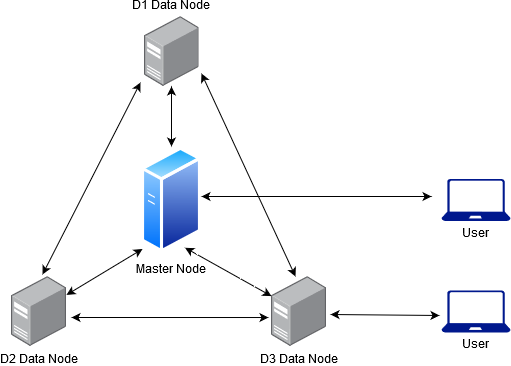
\includegraphics[width=0.35\textwidth]{images/thesis1.png} 
\end{figure}

%CID: Explain briefly each figure

\begin{figure}[h]
\caption{POST: Uploading a sequence to the master node}
\centering
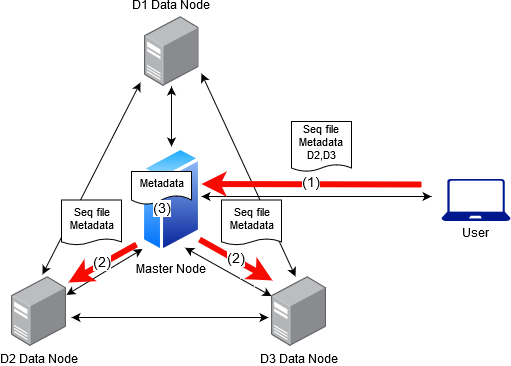
\includegraphics[width=0.35\textwidth]{images/thesis3.png} 
\end{figure}

\begin{figure}[h]
\caption{POST: Uploading a sequence to the data node}
\centering
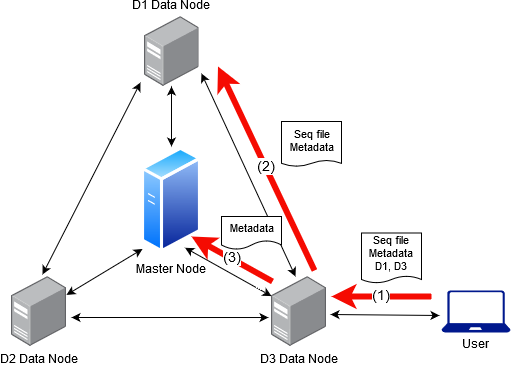
\includegraphics[width=0.35\textwidth]{images/thesis2.png} 
\end{figure}

\begin{figure}[h]
\caption{GET: Downloading a sequence}
\centering
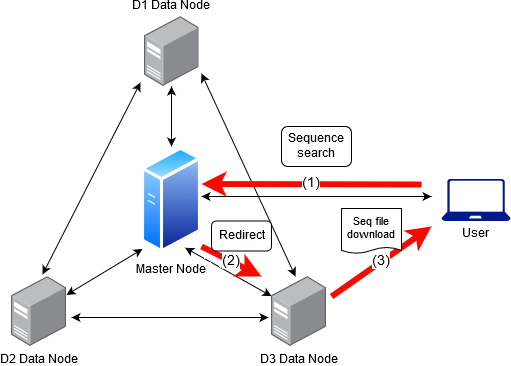
\includegraphics[width=0.35\textwidth]{images/thesis4.png} 
\end{figure}

%CID: Explain the data model and data permissions

%CID: Data Model, make sure to cite this in a paragraph

\begin{table}[h]
\caption{Data Model to be Used in the System}

\begin{tabular}{c|c}
\hline
    key & description \\
\hline
\hline
    seq\textunderscore id & unique ID assigned to all sequences \\
    organism & organism where the sequence was extracted from \\
    quality & the rating of the data based on the number of downloads or another criteria \\
    uploader & user that uploaded the data \\
    institute & institute where the uploader or sequence was taken from \\
    upload\textunderscore date & date the data was uploaded to the database \\
    last\textunderscore modified & the date the metadata or data was edited \\
    data\textunderscore nodes & list of data nodes that this data is contained to
    

\end{tabular}
\label{table:data_model_table}

\end{table}

Table~\ref{table:data_model_table} on Page~\pageref{table:data_model_table} aims to show the metadata that will be initially stored in the database.

%CID: Data Permissions

\begin{table}[h]
\caption{Data Permissions and Users in the System}
\begin{tabular}{c|c}
\hline
    user & description \\
\hline
\hline
   Moderator & Has ability to upload, download, store data, verify \\
    Peer & Has ability to upload, download, store data \\
    Guest & Has ability to upload, download \\
    

    
\end{tabular}
\label{table:data_perm_table}
\end{table}

Table~\ref{table:data_perm_table} on Page~\pageref{table:data_perm_table} shows the different set of users and the permissions allowed to them in the system. The moderator is a special user who has the ability to not allow some data to be uploaded. This is to make sure there is a means to verifying the data being uploaded. All users can upload, download, and store (or host) data. All other users, which are called guests has an ability to download and upload data.


\section{Proposed Methodology}

% CID: explain the 3 main phases (system creation, testing, documentation)
% CID: explain the importance of each phase
% CID: explain

\subsection{Creating the system}
The system will be needed to be done before any of the following steps can occur. 
\begin{enumerate}
    \item Set-up database architecture
    \item Code the POST API
    \item Code the DELETE API
    \item Code the PUT API
    \item Code the GET API
    \begin{enumerate}
        \item As a classic database
        \item Revise to have distributed database functionality (may be moved to item 1) 
        \begin{enumerate}
            \item Code data node
            \item Deploy \& test functionality of data node/s
            \item Code master node
            \item Deploy \& test functionality of master node/s
            \item Test interoperability of nodes
        \end{enumerate}
    \end{enumerate}
\end{enumerate}

\subsection{Testing}
Part of the goal of the project is to implement a better data transfer mechanism. And one way to verify this is to see the speed in which the system compares to other systems.

\begin{enumerate}
    \item Create test for testing original speed
    \item Test original download speeds
    \item Create test for testing new speed
    \item Test new speeds
\end{enumerate}


\subsection{Documentation}
Another part of this project's goal as well is to make this available and usable for the community. And documentation will help make the system easy to use, manage, and develop.
\begin{enumerate}
    \item Compiled to a PDF that is easy to read
    \item How to use (all users)
    \item How to set up
    \item How to maintain and add features
\end{enumerate}

\subsection{Resources needed}

Servers must have networking capability and at the very least have their HTTP port configured to be open to each other, or optionally, the HTTP port can be open to the Internet.
\begin{enumerate}
    \item 1-2 servers in PGC to serve as master node (1 minimum; the other server will serve as data node)
    \item 1-2 servers in DCS to serve as data nodes (1 minimum)
    \item 2 workstations where both of us can program the system
    \end{enumerate}
\end{enumerate}

\printbibliography

\end{document}